\documentclass{beamer}
\usepackage{animate}

\usepackage[T1]{fontenc}
%\usepackage{arevtext,arevmath}
%\usepackage{ccfonts} 
\usepackage[utf8]{inputenc}
%\usepackage[italian]{babel}
\usetheme{Rochester}
\usefonttheme[onlymath]{serif}
\usepackage{diffcoeff}
\usepackage{graphicx}
\usepackage{bm}
\usepackage{amsmath}
\usepackage{amssymb}
\usepackage{wrapfig}
\usepackage{amsfonts}
\usepackage{amsthm}
\usepackage{amscd}
\usepackage{multicol}
\usepackage{tikz}
\newenvironment{sistema}%
{\left\lbrace\begin{array}{@{}l@{}}}%
{\end{array}\right.}

\title{Modelling cell differentiation using stochastic dynamical systems on
graphs}%\author{Riccardo Scheda \\ %\flushleft{Relatore: Prof. Armando Bazzani}}
\institute[]{\\University of Bologna}
\author{\Large{Riccardo Scheda}}
\date{1 October 2020}


\begin{document}

\begin{frame}
\maketitle
\end{frame}


\begin{frame}
\frametitle{Waddington potential}

\begin{figure}[h]
\centering
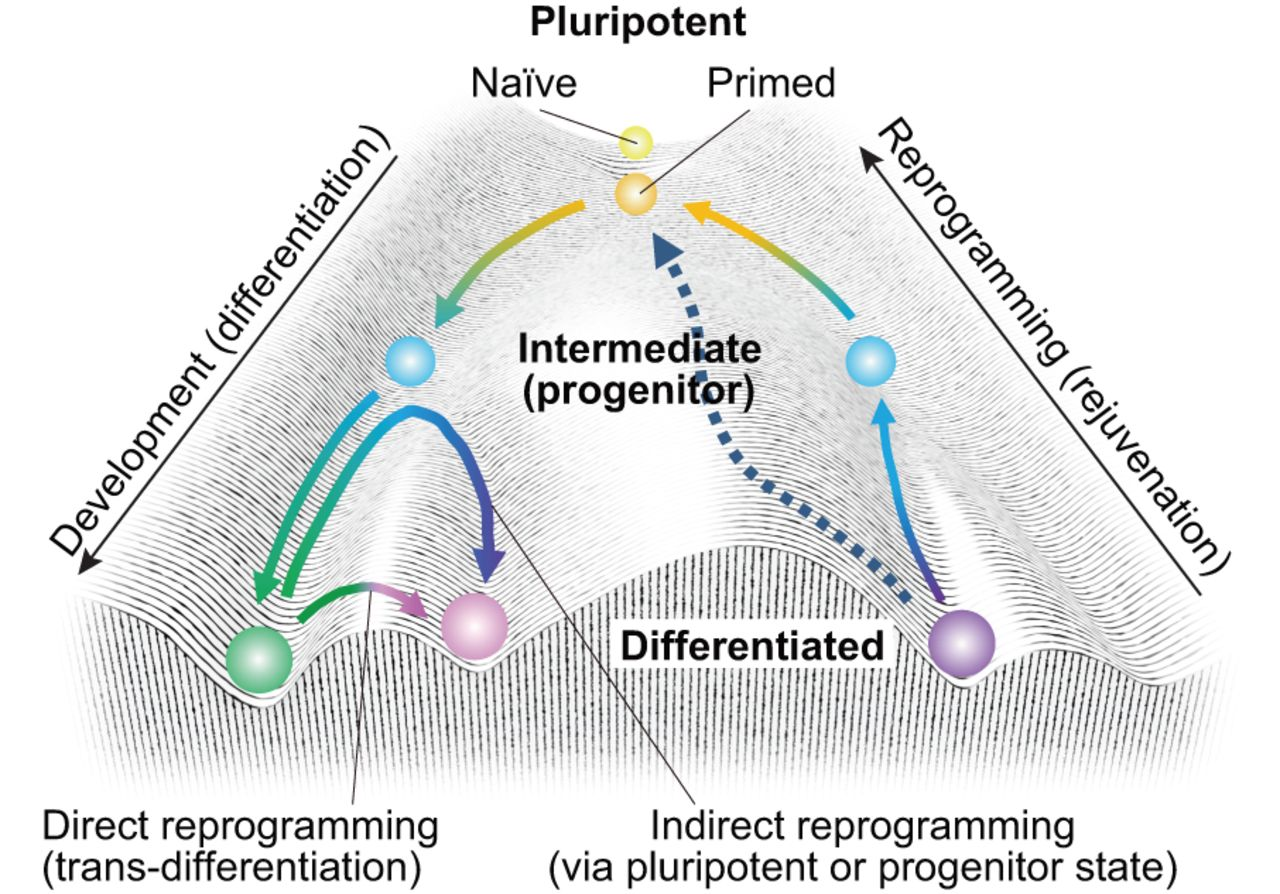
\includegraphics[scale=1]{landscape.jpg}
\end{figure}
\end{frame}



\begin{frame}
\frametitle{Introduction - Gene Regulatory Networks}
Gene Regulatory Networks for cell differentiation

\begin{figure}[h]
\centering
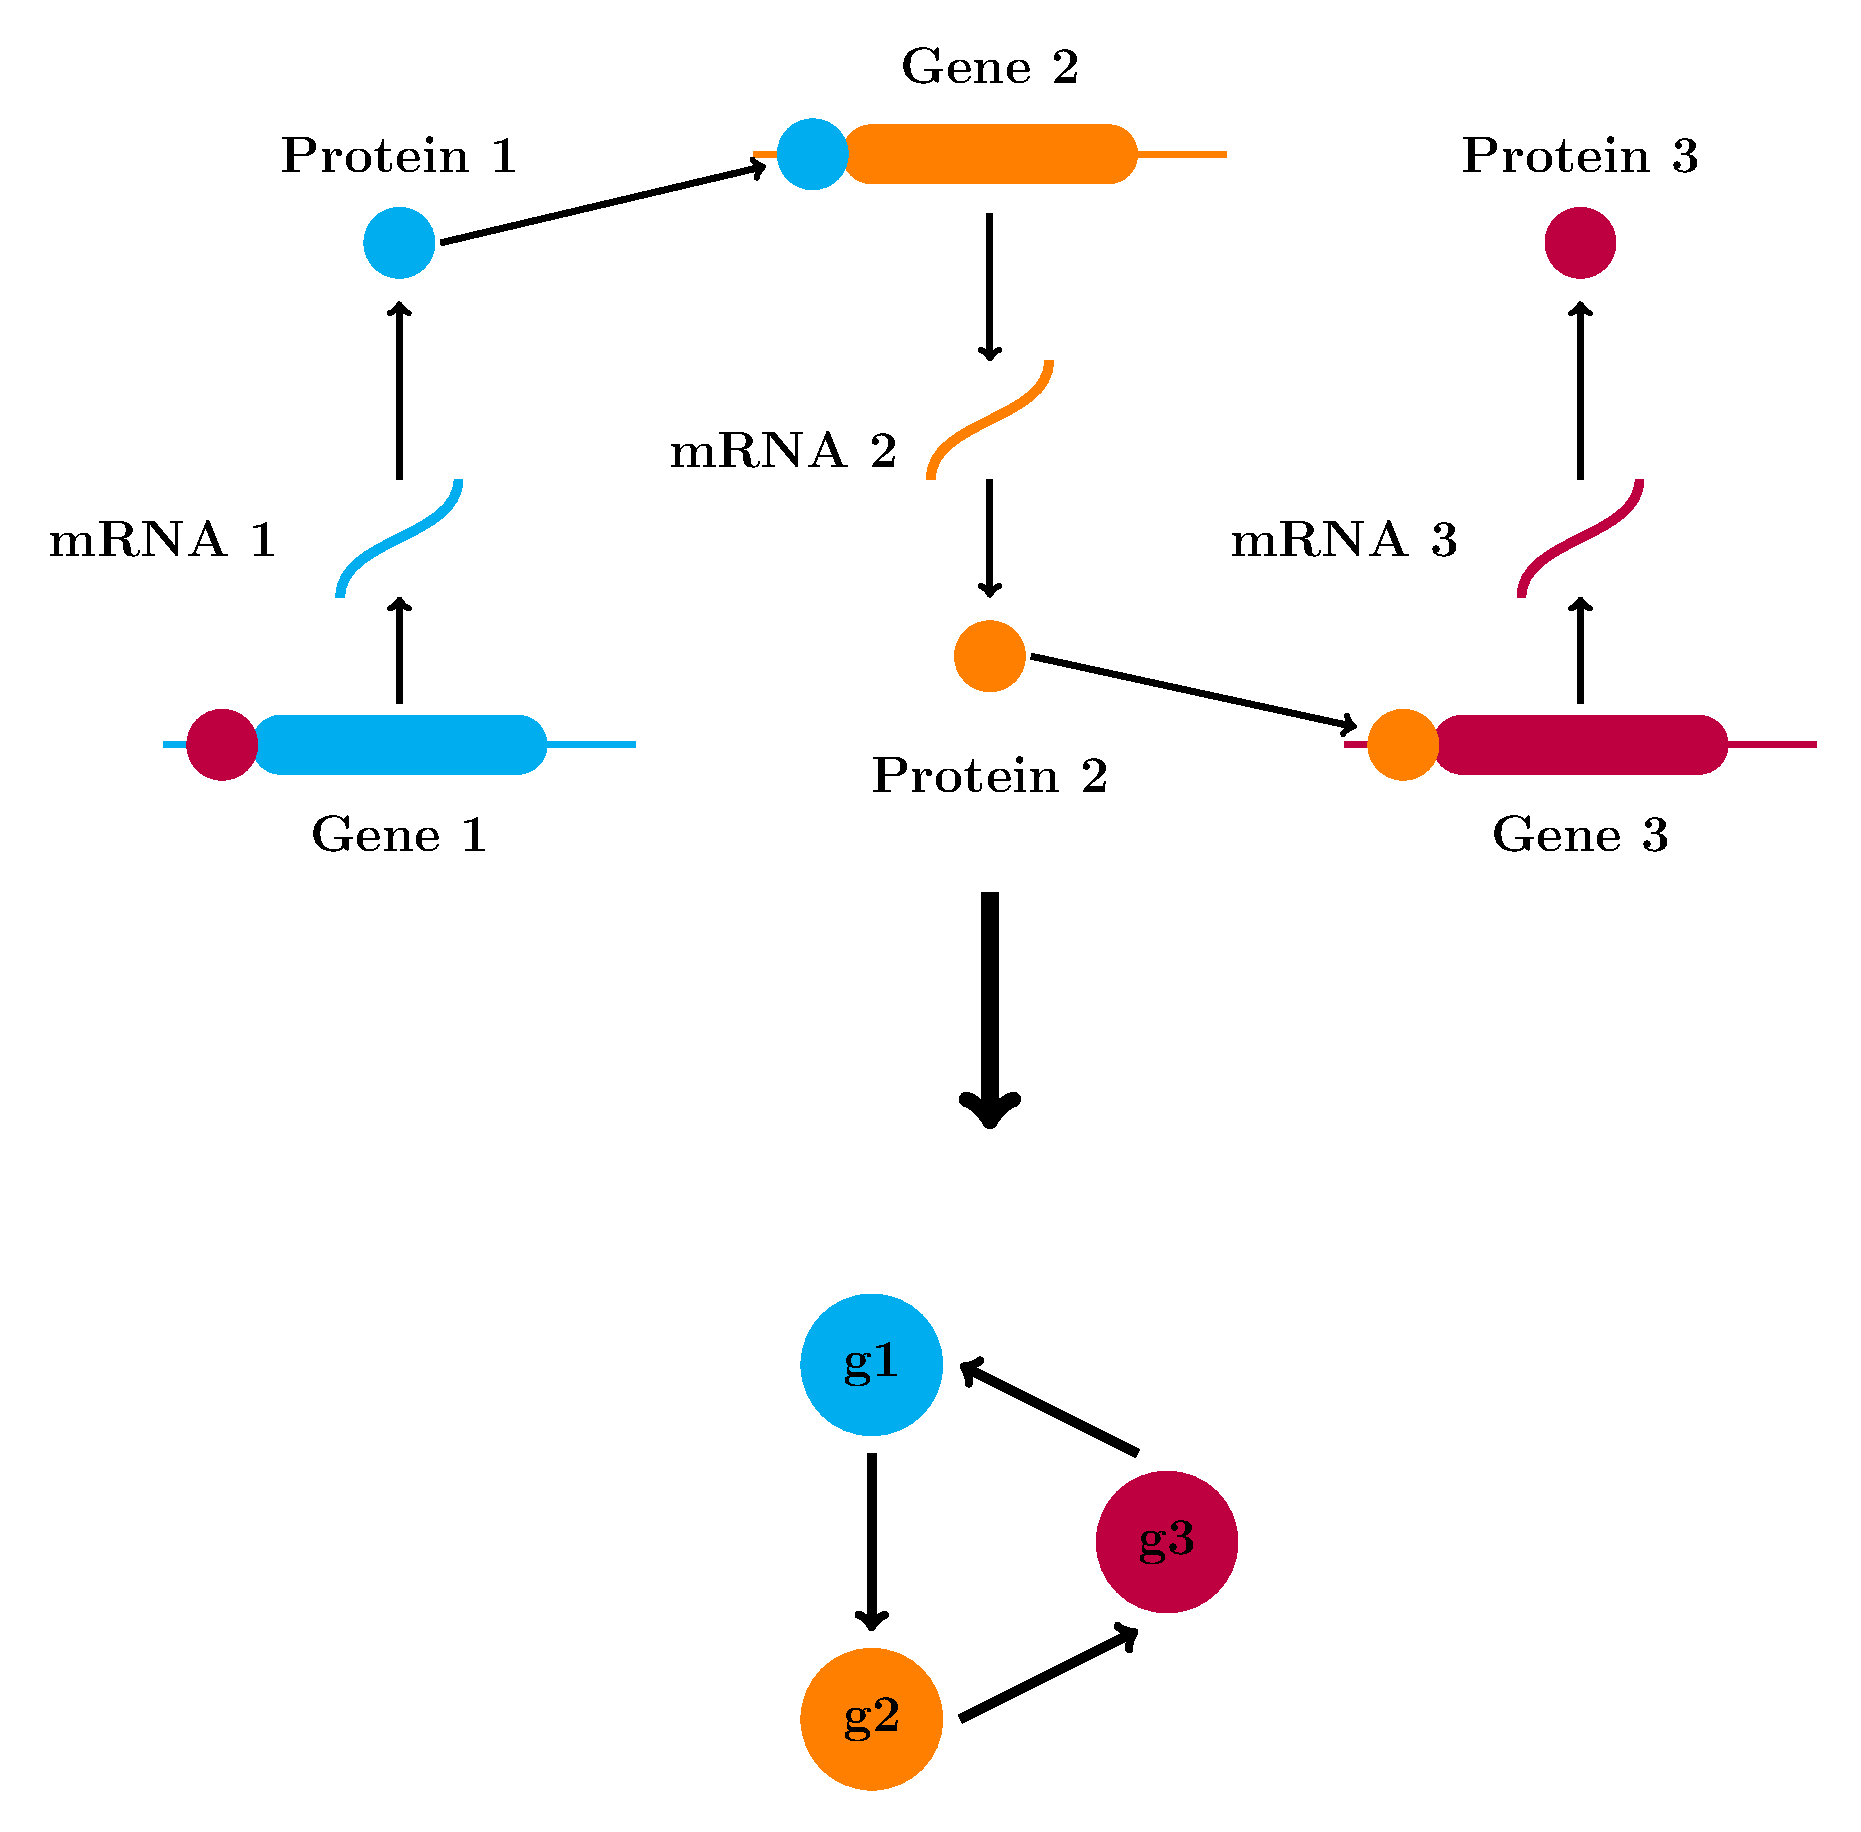
\includegraphics[scale=0.2]{images/grnn.pdf}
\end{figure}
\end{frame}

\begin{frame}


\frametitle{Random Boolean Networks}
Random Boolean Networks are networks in which each node can have only the values 0 or 1:
$$
\sigma_i(t) \in \{0,1\}
$$
And the discrete evolution of the network is given by:
$$
\sigma_i(t+1)=\Phi_i(\sigma(t))=\Theta\left (\sum_j A_{ij}\sigma_j(t)\right )
$$
where $A$ is the connectivity matrix and $\Theta(x)$ is the Heaviside function.
\end{frame}

\begin{frame}
\frametitle{Random Boolean Networks}
\begin{figure}[h]
\centering
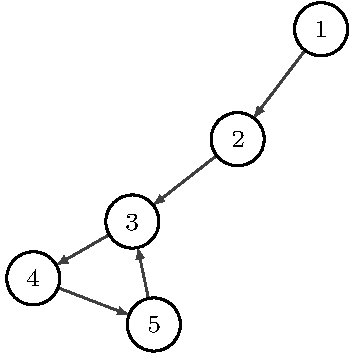
\includegraphics[scale=0.5]{images/singlecluster.pdf}
\end{figure}
The connectivity matrix $A$ of this network will be constructed as follows:
$$
A = \left (
\begin{array}{ccccc}

0 & 0 & 0 & 0 & 0  \\
1 & 0 & 0 & 0 & 0  \\
0 & 1 & 0 & 0 & 1  \\
0 & 0 & 1 & 0 & 0  \\
0 & 0 & 0 & 1 & 0  \\

\end{array}
\right )
$$
\end{frame}


\begin{frame}
\frametitle{The model - Deterministic Evolution}
Deterministic evolution of the activity:
\begin{figure}
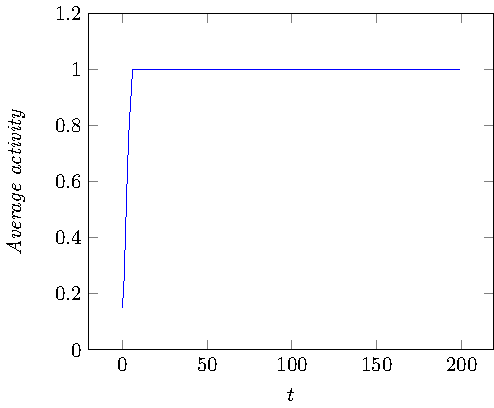
\includegraphics[scale = 0.8]{images/det.pdf}
\end{figure}
\end{frame}


\begin{frame}
\frametitle{Discrete evolution}
The system is deterministic, but during the evolution we can add noise to the system:
\begin{enumerate}
\item internal noise, which hinibits the activation of the nodes
\item envinromental noise, which can activate some nodes in the network
\end{enumerate}

\begin{figure}
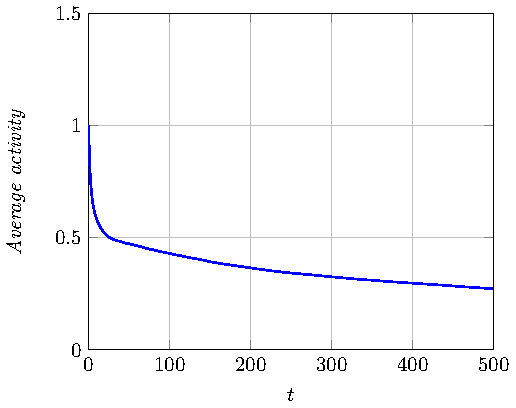
\includegraphics[scale = 0.6]{images/n.pdf}
\end{figure}
\end{frame}


\begin{frame}
\frametitle{The model - Multiple cluster networks}
We can construct networks with multiple clusters 
\begin{figure}
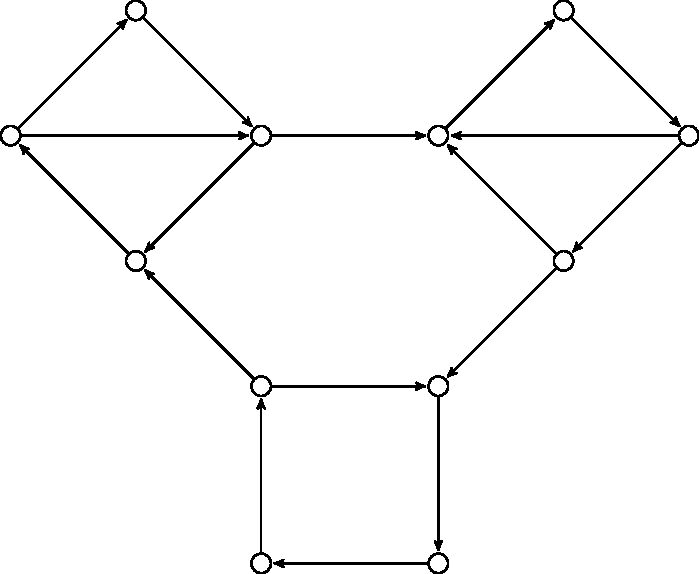
\includegraphics[scale=0.7]{grn1.pdf}
\end{figure}
\end{frame}




\begin{frame}
\frametitle{The model - Double-cluster networks}
In this work we consider networks made by two clusters which hinibit each other:
A subnetwork hinibits the other: 
\begin{figure}
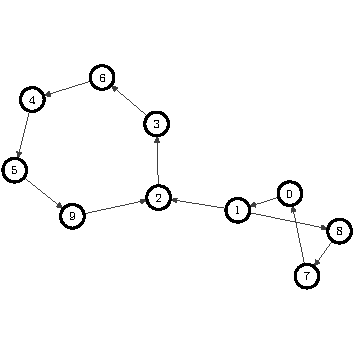
\includegraphics[scale=0.8]{prova.pdf}
\end{figure}
The two clusters are connected by negative links.
\end{frame}


\begin{frame}
\frametitle{Double-cluster networks}
We can introduce a metadynamics where $\nu_k(t)$ is the state of the $k$ subnetwork and
we have a relation
$$
\nu_k(t+\Delta t)-\nu_k(t)=\phi(\nu_k(t))-\gamma\left (H_{kj}\nu_j(t)\right )
$$
\begin{figure}
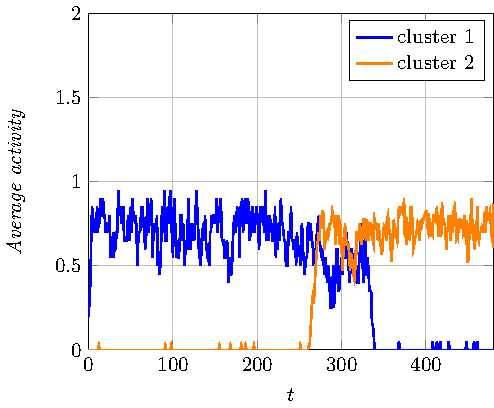
\includegraphics[scale=0.8]{images/metad.pdf}
\end{figure}
\end{frame}



\begin{frame}
\frametitle{Kramer Transition Rate Theory}
$$
dx = -V'(x)dt + \sqrt{2T} dw_t
$$
\begin{figure}
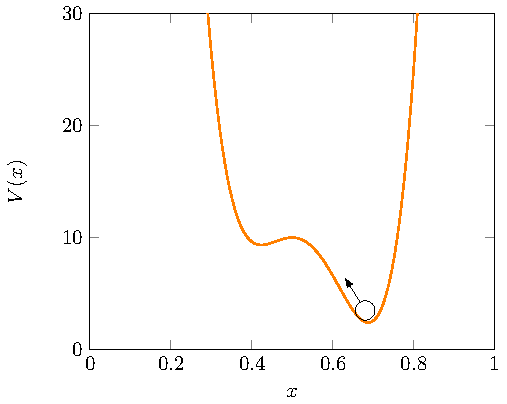
\includegraphics[scale=0.5]{images/kramerwell.pdf}
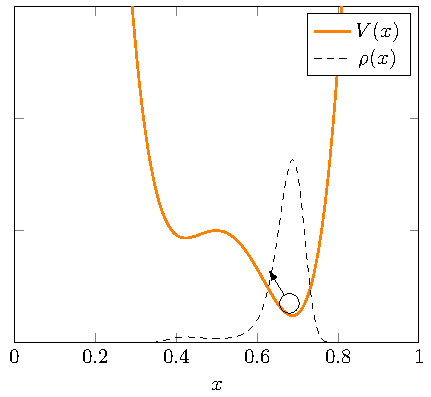
\includegraphics[scale=0.5]{images/kramerpot.pdf}

\end{figure}
$$
k_{a\to c} \simeq \frac{\omega_a \omega_b}{2 \pi} e^{\frac{V_b-V_a}{T}}
$$
So the log of transition rates gives us an estimate for the potential $V(x)$.
\end{frame}


\begin{frame}
\frametitle{The model related to Kramer Theory}
Given an ensemble of double-cluster networks, we can make an estimate for a double well potential: The local minima of the potential are the stationary states of the two clusters of the networs. We expect that the potential $V$ depends on the size and on the number of links per node:
$$
V = V(N,K)
$$
\end{frame}


\begin{frame}
\frametitle{Ensemble}
To measure the activity transition, we can define the total activity of the network:
$$
I(t) = \nu_2(t) - \nu_1(t)
$$
with $\nu_k(t) \in [0,1]$ and $I(t) \in [-1,1]$.
Starting from an initial condition in which only the second  cluster is active:
$$
\rho_0(I) = \delta(I-1)
$$
Every time the activity passes from one cluster to the other, we register the time of transition.
\end{frame}

\begin{frame}
\frametitle{Evolution of the system}
\begin{figure}
\centering
\animategraphics[scale=0.8,autoplay,loop]{10}{images/gif/graph}{0}{99}
\end{figure}
\end{frame}

\begin{frame}
\frametitle{Transition times}

\begin{figure}
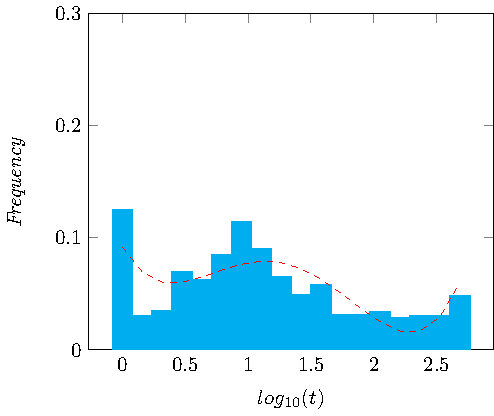
\includegraphics[scale=0.8]{images/fittimes.pdf}
\end{figure}

The histogram of transition rates (in logarithmic scale) shows a possible form of the potential for the double-cluster networks.
\end{frame}




\end{document}




